\chapter{Marco teórico}\label{sec:marcoteorico}
%se presenta, se discute, se revisa, se dedica a, tal tiene la intención de recordar conceptos, 
\section{Robots bípedos}
Un robot bípedo es un tipo de robot móvil que cuenta con dos piernas, y su principal diferencia entre otros es su locomoción bípeda. \cite{yang2017stateart} El ejemplo más común y concreto de esta clasificación son los robots humanoides. La investigación en este campo ha tenido lugar desde la década de 1960, cuando RSmo-sher de American General Corporation produjo el primer robot de caminata bípeda, Rig. Este hito marcó el inicio de la investigación en robots humanoides, siendo el científico yugoslavo M. Vukobratovic quien propuso en 1969 la base para esta área: el criterio de estabilidad Zero Moment Point (ZMP).\cite{chen2013walking}
El transcurso del desarrollo de estas investigaciones ha tenido lugar alrededor del mundo. Japón tiene una posición prominente, una de las mayores contribuciones ha sido el trabajo de Honda con los modelos ASIMO (a) y P3 (b) que llevaron este campo a otro nivel.\cite{chen2013walking}
\begin{figure}[H]
	\centering
	\begin{subfigure}[b]{0.5\textwidth}
		\centering
		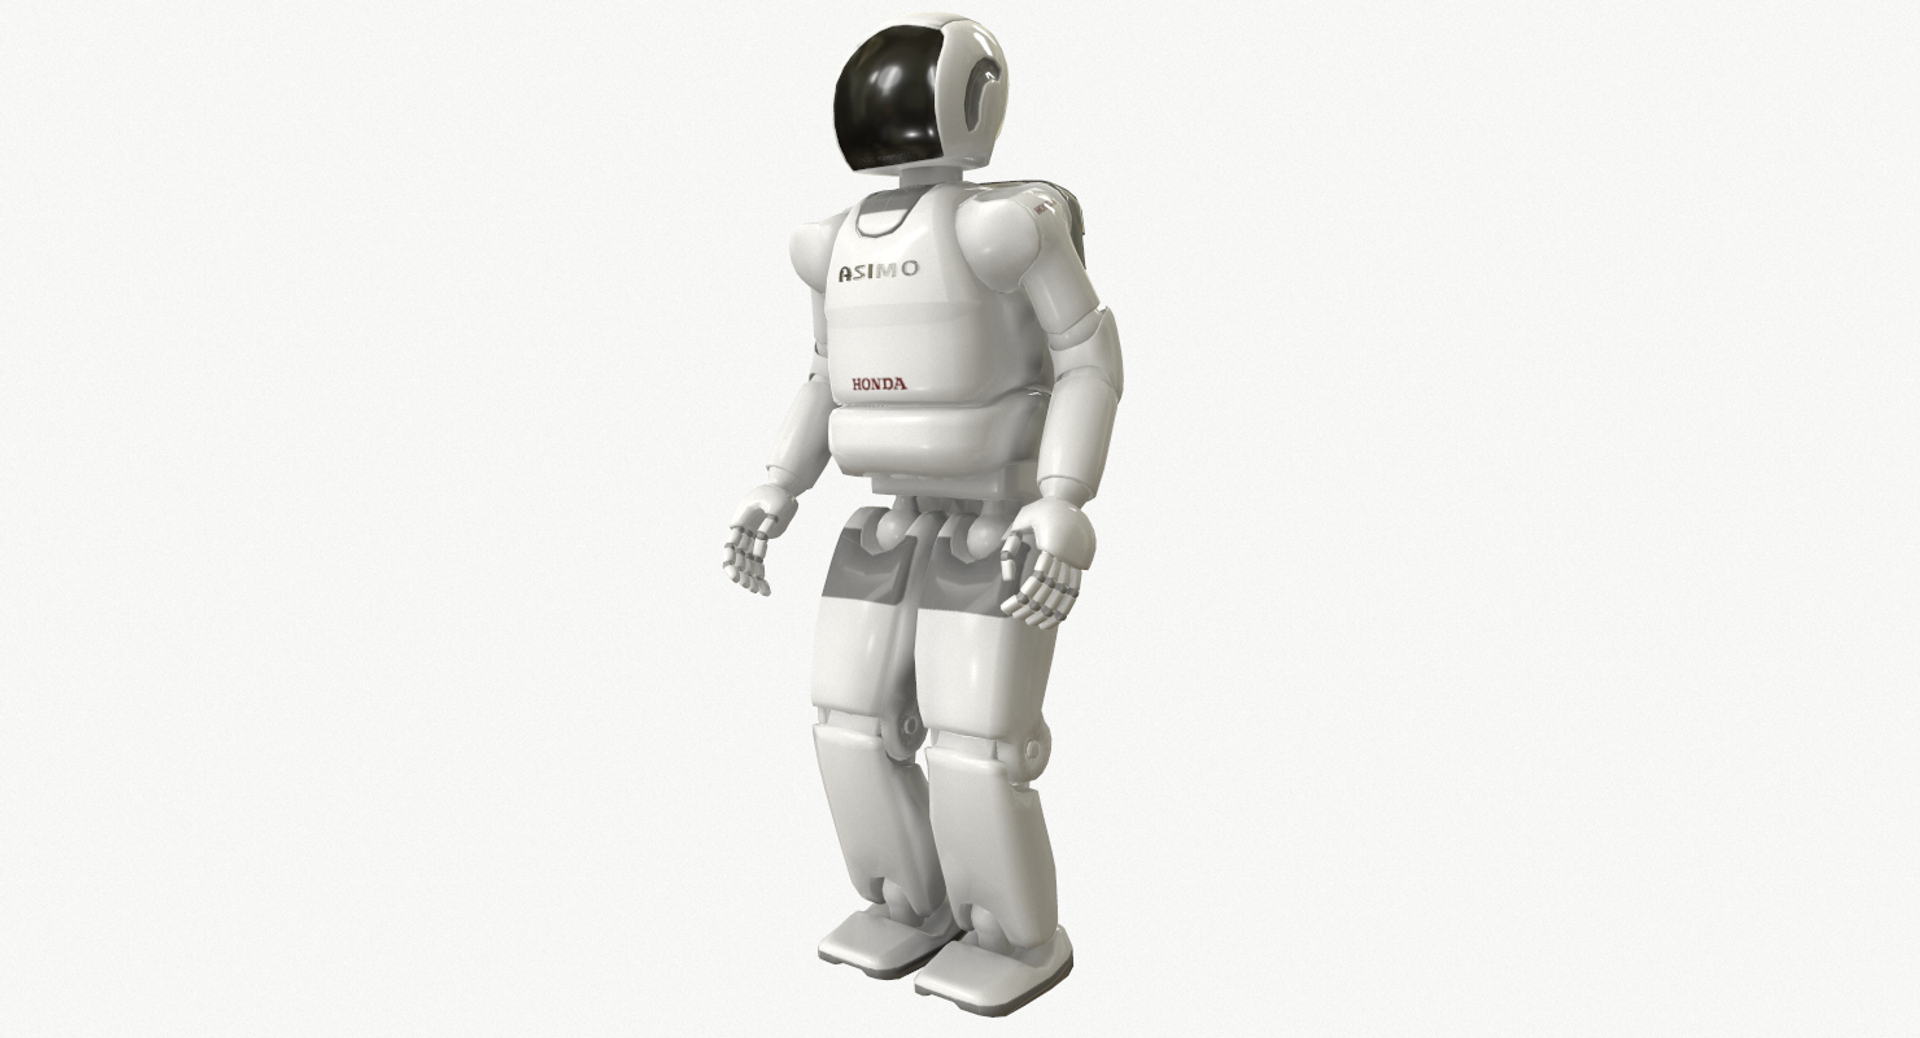
\includegraphics[width=\textwidth]{images/ASIMO.jpg}
		\caption{ASIMO Robot}
		\label{fig:image1}
	\end{subfigure}
	\hfill
	\begin{subfigure}[b]{0.24\textwidth}
		\centering
		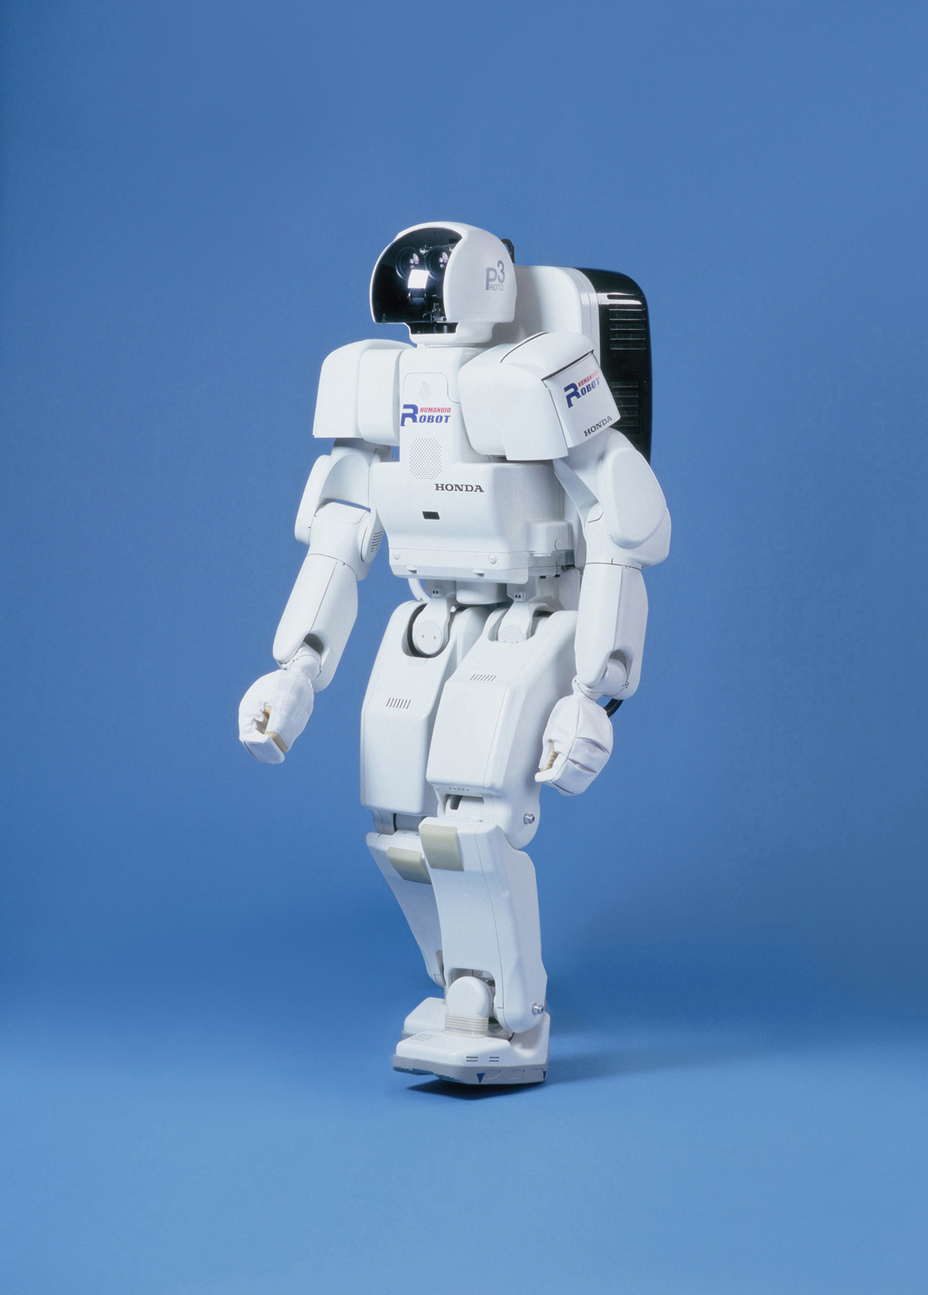
\includegraphics[width=\textwidth]{images/P3_robot.jpg}
		\caption{P3 Robot}
		\label{fig:image2}
	\end{subfigure}
	\caption{P3 Robot fue el primer bípedo humanoide completamente independiente, completado en Septiembre de 1997}
	\label{fig:parallel_images}
\end{figure}
<<<<<<< HEAD
=======

>>>>>>> 0606a29eeae5d0a18979d21ddf9bcba11f909db4

\section{Conceptos básicos de visión artificial} 
%Un párrafo para cada espaico de color 
Aunque la visión artificial es un campo muy extenso, en términos generales, se trata de la transformación de datos obtenidos de cámaras, ya sea en forma de imágenes fijas o secuencias de video. A partir los datos de entrada se extrae información contextual y con ello una decisión; como encontrar objetos en una escena, o nueva representación; como pasar una imagen a color a blanco y negro. La capacidad de entender el mundo visual es un requisito para una máquina inteligente. \cite{bradski2008learning} Por ello, este campo es de suma importancia en la robótica, le permite a un robot ser autónomo, navegar, interactuar con el entorno y realizar múltiples tareas. \\Existen herramientas que facilitan la implementación de estas capacidades ya que proporcionan diversos algoritmos y funciones para aplicaciones de visión.\\
OpenCV es una biblioteca de visión por computadora ampliamente utilizada, diseñada para la eficiencia computacional y con un fuerte enfoque en aplicaciones en tiempo real \cite{bradski2008learning}. 

Algunas técnicas y algoritmos utilizados en este trabajo:

\begin{itemize}
	\item \textbf{Detección y extracción de características}
\end{itemize}

\section{Redes neuronales artificiales}
    
\section{Competencia Robocup Humanoid kid size}
  ´